\documentclass[a4paper,11pt]{article}
\usepackage[slovene]{babel}
\usepackage[utf8]{inputenc}
\usepackage{graphicx}
\usepackage{hyperref}
\usepackage{listings}
\usepackage{geometry}
\geometry{margin=1in}

\title{\textbf{Računalniške Storitve v Oblaku - Poročilo} \newline Extreme Weather Event Notifier}
\author{Projektna ekipa 19, Jaka Škerjanc in Erik Pahor}
\date{\textbf{2025}}

\begin{document}

\maketitle

\newpage

\section*{Povezava do repozitorija kode}
Projektna koda je dostopna na javno dostopnem repozitoriju GitHub, kar omogo\v{c}a vpogled v implementacijo ter CI/CD konfiguracijo:
\begin{itemize}
	\item Repozitorij: \url{https://github.com/rso2425/extreme-weather-event-notifier}
	\item Aplikacija: \url{https://rso-weather.duckdns.org/}
\end{itemize}

\section*{Kratek opis projekta}
Extreme Weather Event Notifier je spletna aplikacija, ki uporabnike obve\v{s}\v{c}a o ekstremnih vremenskih dogodkih v Sloveniji. Uporabniki lahko omogo\v{c}ijo prejemanje potisnih obvestil in dostopajo do zgodovine vremenskih dogodkov. Aplikacija zbira podatke iz Agencije Republike Slovenije za okolje (ARSO) in jih obdeluje v mikrostoritvenem sistemu. Potisna obvestila se po\v{s}iljajo preko Firebase Cloud Messaging, podatki pa se shranjujejo v MongoDB in so dostopni preko spletnega vmesnika.

\section*{Ogrodje in razvojno okolje}
Pri razvoju projekta so bili uporabljeni sodobni jeziki in orodja, ki omogo\v{c}ajo skalabilno in vzdr\v{z}evalno infrastrukturo:
Frontend je implementiran s pomo\v{c}jo Nuxt.js, za backend pa se uporablja Express.js. Podatki se shranjujejo v MongoDB, medtem ko RabbitMQ slu\v{z}i za medstoritveno komunikacijo. Infrastruktura temelji na Dockerju in Kubernetesu, CI/CD procesi pa so avtomatizirani s pomo\v{c}jo GitHub Actions.
\newpage
\section*{Arhitektura sistema}
Arhitektura aplikacije temelji na mikrostoritvenem modelu, kjer vsaka storitev izpolnjuje dolo\v{c}eno funkcijo:
\begin{figure}[h!]
	\centering
	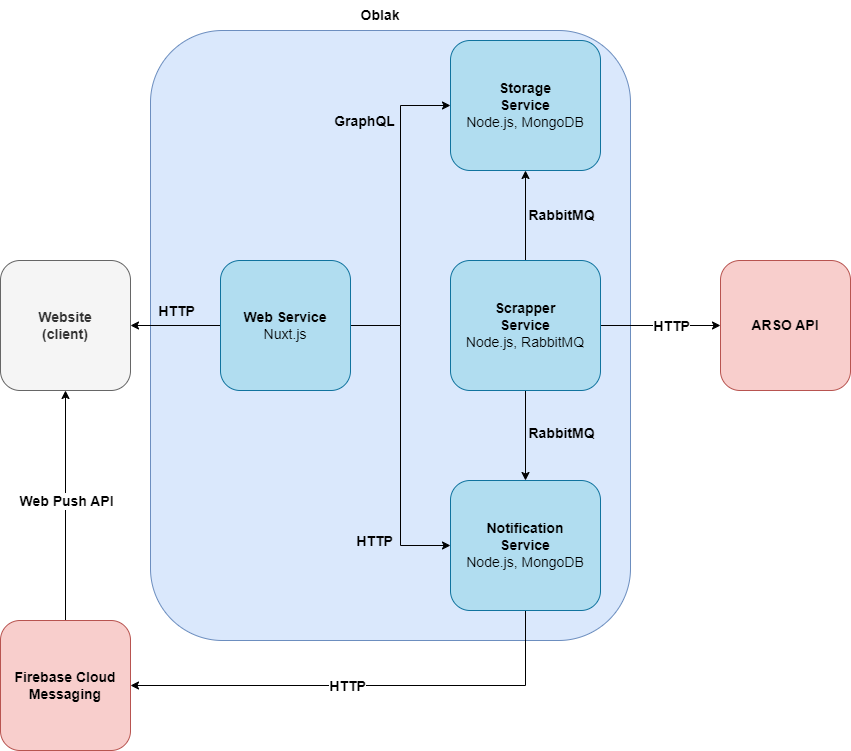
\includegraphics[width=\textwidth]{images/architecture.png}
	\caption{Shema arhitekture aplikacije}
\end{figure}

Aplikacija sestavljajo \v{s}tiri glavne mikrostoritve: Web, Notification, Scraper in Storage. Komunikacija med storitvami poteka preko RabbitMQ in API-jev (REST in GraphQL). Push obvestila se po\v{s}iljajo preko Firebase Cloud Messaging.

\section*{Opis mikrostoritev}
\subsection*{Web Mikrostoritev}
Web mikrostoritev predstavlja uporabni\v{s}ki vmesnik aplikacije, implementiran v Nuxt.js. Uporabnikom omogo\v{c}a:

- Pregled zgodovine vremenskih dogodkov, ki se pridobijo iz Storage mikrostoritve preko GraphQL.

- Prijavo in odjavo na potisna obvestila preko Notification mikrostoritve.

- Upravljanje potisnih obvestil s Firebase Cloud Messaging.

\subsection*{Notification Mikrostoritev}
Notification mikrostoritev je odgovorna za po\v{s}iljanje potisnih obvestil in upravljanje Firebase ID-jev uporabnikov. Prejema dogodke iz Scraper mikrostoritve preko RabbitMQ in po\v{s}ilja obvestila uporabnikom z registriranimi napravami.

\subsection*{Scraper Mikrostoritev}
Scraper mikrostoritev periodi\v{c}no zbira podatke o vremenskih dogodkih iz ARSO preko CAP XML standarda. Ti podatki se obdelujejo in po\v{s}iljajo Notification ter Storage mikrostoritvama preko RabbitMQ.

\subsection*{Storage Mikrostoritev}
Storage mikrostoritev shranjuje podatke o vremenskih dogodkih v MongoDB in izpostavlja GraphQL API, ki omogo\v{c}a pridobivanje podatkov za prikaz zgodovine dogodkov v Web mikrostoritvi.

\section*{Primeri uporabe}
Aplikacija omogo\v{c}a uporabniku enostavno interakcijo:
Uporabnik obi\v{s}\v{c}e spletno mesto, omogo\v{c}i potisna obvestila, in prejme Firebase ID, ki je shranjen v Notification mikrostoritvi. Scraper zazna vremenski dogodek, ki se po\v{s}lje v RabbitMQ. Notification po\v{s}lje obvestilo uporabnikom, Storage pa omogo\v{c}a vpogled v zgodovino dogodkov.

\section*{Seznam opravljenih projektnih zahtev}
\begin{itemize}
	\item \textbf{Repozitorij}
	      
	      \begin{itemize}
	      	\item Ustvarjen GitHub repozitorij dostopen na \href{https://github.com/rso2425/extreme-weather-event-notifier}{rso2425/extreme-weather-event-notifier}.
	      	\item Ustvarjena je datoteka README.md, ki opisuje projekt (\href{https://github.com/rso2425/extreme-weather-event-notifier/blob/main/README.md}{README.md}).
	      	\item Dodana je omejitev na glavno vejo, spremembe so možne le preko pull requestov in razvijalske veje.
	      \end{itemize}
	      
	      \begin{figure}[ht!]
	      	\centering
	      	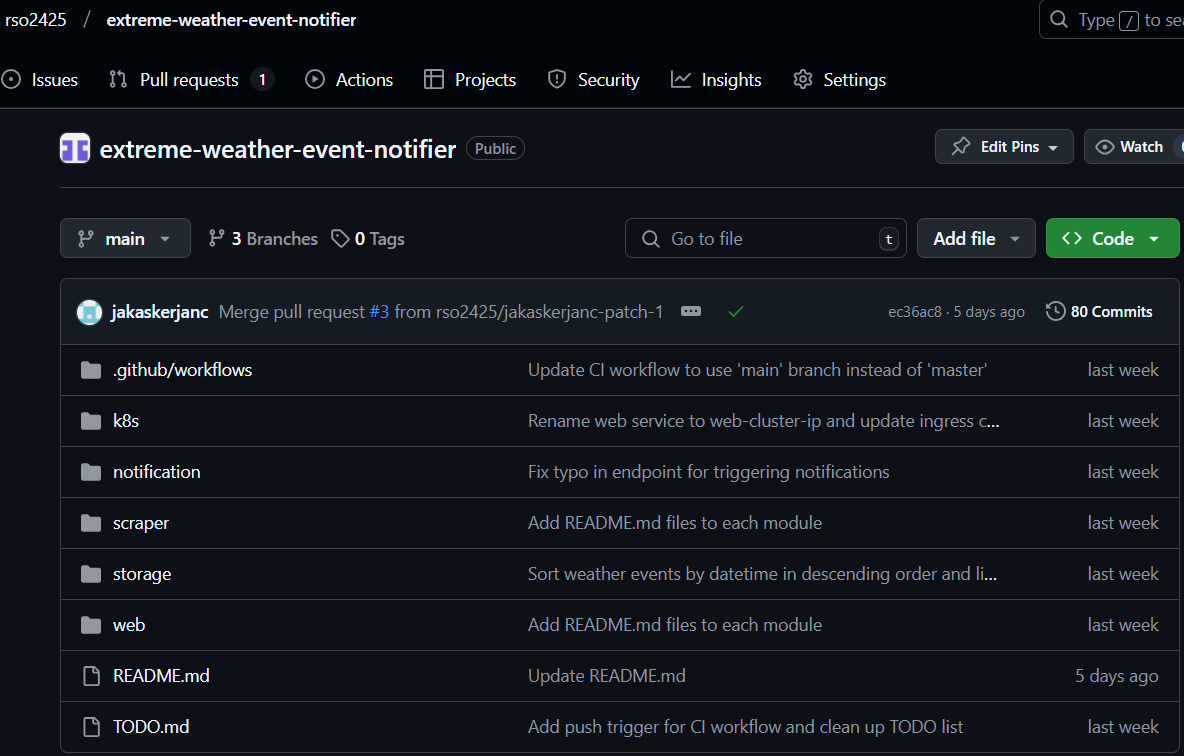
\includegraphics[width=0.7\textwidth]{images/repo.png}
	      	\caption{Struktura repozitorija}
	      	\label{fig:repo}
	      \end{figure}
	              
	\item \textbf{Mikrostoritve in »cloud-native« aplikacija}
	      \begin{itemize}
	      	\item Vsaka mikrostoritev je v svojem direktoriju.
	      	\item Vsaka mikrostoritev ima implementirana navodila za namestitev in zagon.
	      	\item Storitve komunicirajo prek HTTP in RabbitMQ sporočilnega protokola.
	      	\item Vsaka storitev ima svoje Kubernetes manifeste.
	      	\item Uporabljena je MongoDB NoSQL podatkovna baza, z nekaj podatkih o vremenskih dogodkih.
	      \end{itemize}
	\item \textbf{Dokumentacija}
	      \begin{itemize}
	      	\item Dodan dokument README.md, ki podrobno opisuje projekt. (\href{https://github.com/rso2425/extreme-weather-event-notifier/blob/main/README.md}{README.md})
	      \end{itemize}
	\item \textbf{Dokumentacija API}
	      \begin{itemize}
	      	\item Javno dostopne končne točke API-jev so dokumentirane z OpenAPI specifikacijo. (\href{https://rso-weather.duckdns.org/docs/tag/api-routes}{Dokumentacija})
	      	\item Dodani so primeri zahtev in odgovorov.
	      \end{itemize}
	      
	      \begin{figure}[h!]
	      	\centering
	      	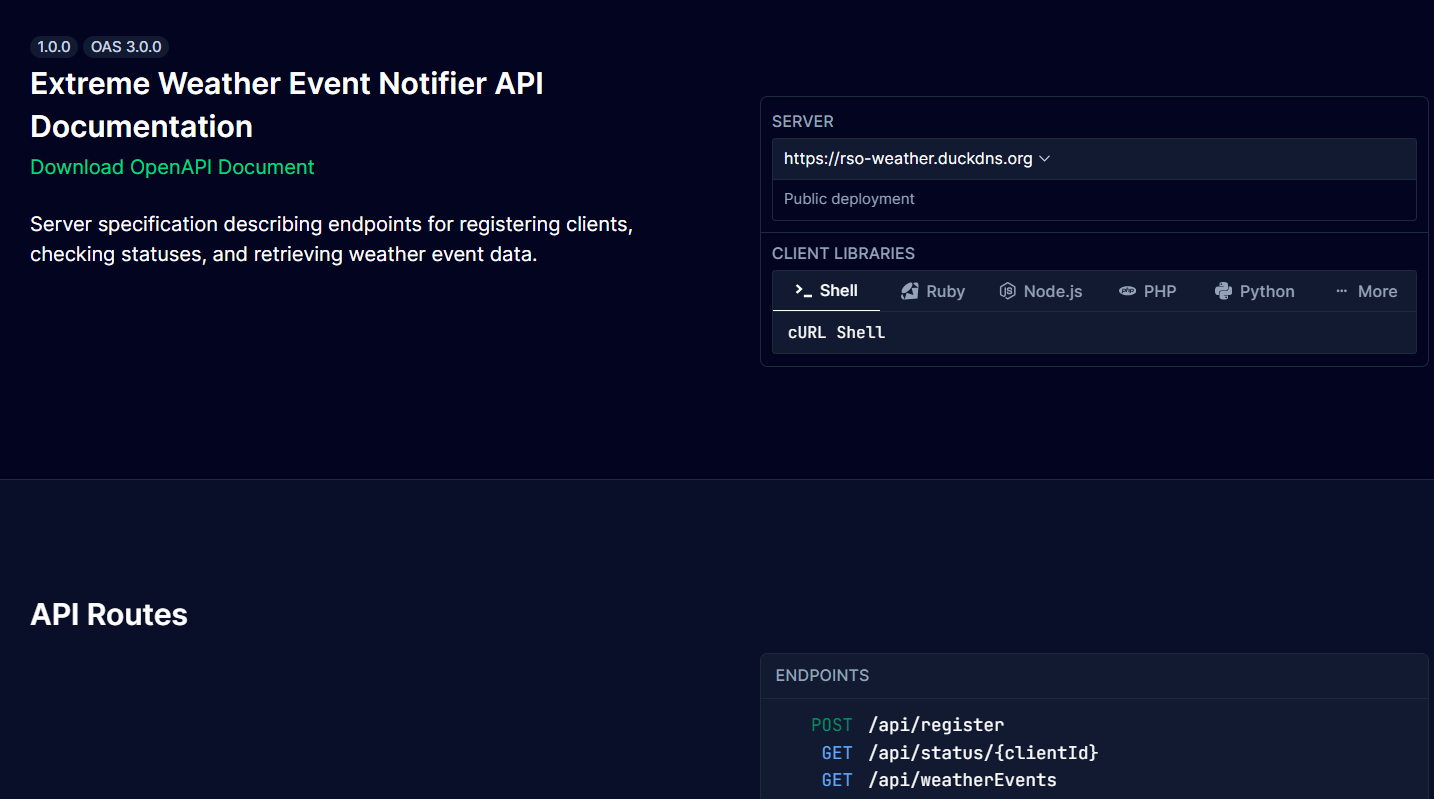
\includegraphics[width=0.7\textwidth]{images/openapi.png}
	      	\caption{Dokumentacija API}
	      	\label{fig:openapi}
	      \end{figure}
	              
	\item \textbf{Cevovod CI/CD}
	      \begin{itemize}
	      	\item Ustvarjen je cevovod CI/CD, ki izvede gradnjo Docker slik, testiranje in namestitev v DigitalOcean.
	      	\item Uporabljen je GitHub Actions za izvedbo cevovoda.
	      	\item Ustvarjena je datoteka .github/workflows/ci.yaml, ki opisuje cevovod. (\href{https://github.com/rso2425/extreme-weather-event-notifier/blob/main/.github/workflows/ci.yaml}{ci.yaml})
	      \end{itemize}
	      
	      \begin{figure}[h!]
	      	\centering
	      	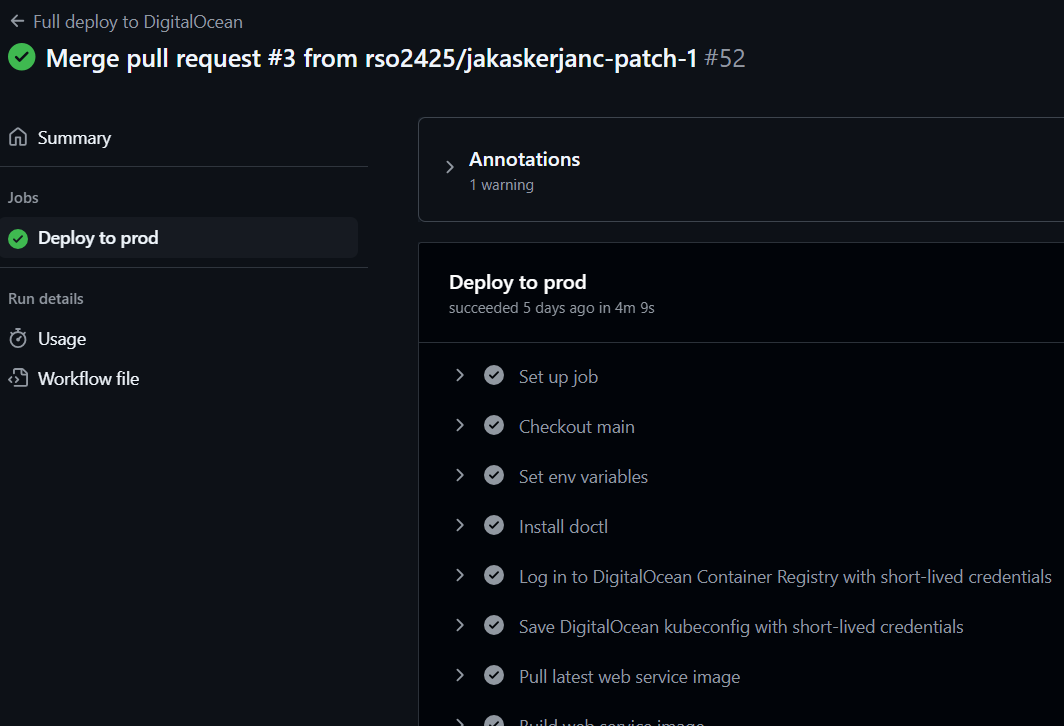
\includegraphics[width=0.7\textwidth]{images/ci.png}
	      	\caption{Cevovod CI/CD}
	      	\label{fig:ci}
	      \end{figure}
	      
	      
	\item \textbf{Namestitev v oblak}
	      \begin{itemize}
	      	\item Ustvarjena je infrastruktura v DigitalOcean.
	      	\item Namestitev je javno dostopna na \href{https://rso-weather.duckdns.org/}{rso-weather.duckdns.org}.
	      \end{itemize}
	      
	      
	      \begin{figure}[h!]
	      	\centering
	      	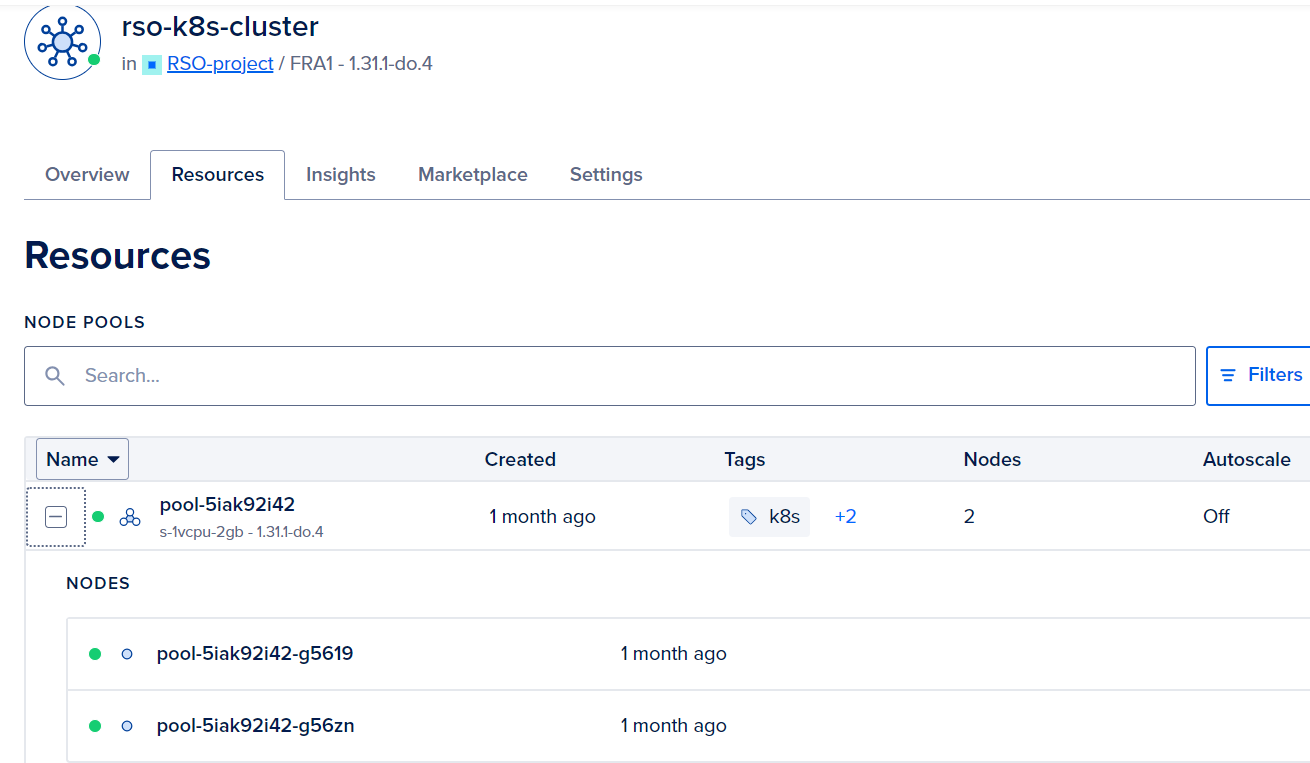
\includegraphics[width=0.7\textwidth]{images/digitalocean.png}
	      	\caption{Infrastruktura v oblaku}
	      	\label{fig:do}
	      \end{figure}
	              
	\item \textbf{Zunanji API}
	      \begin{itemize}
	      	\item Dodan je zunanji API, ki omogoča pridobivanje podatkov o vremenskih dogodkih.
	      	\item ARSO API je javno dostopen zato autentikacija ni potrebna.
	      	\item Uporablja se Firebase Cloud Messaging za pošiljanje potisnih obvestil.
	      	\item Privatni ključi niso shranjeni v repozitoriju ampak se prenesejo v Docker sliko ob gradnji.
	      \end{itemize}
	      
	      \begin{figure}[h!]
	      	\centering
	      	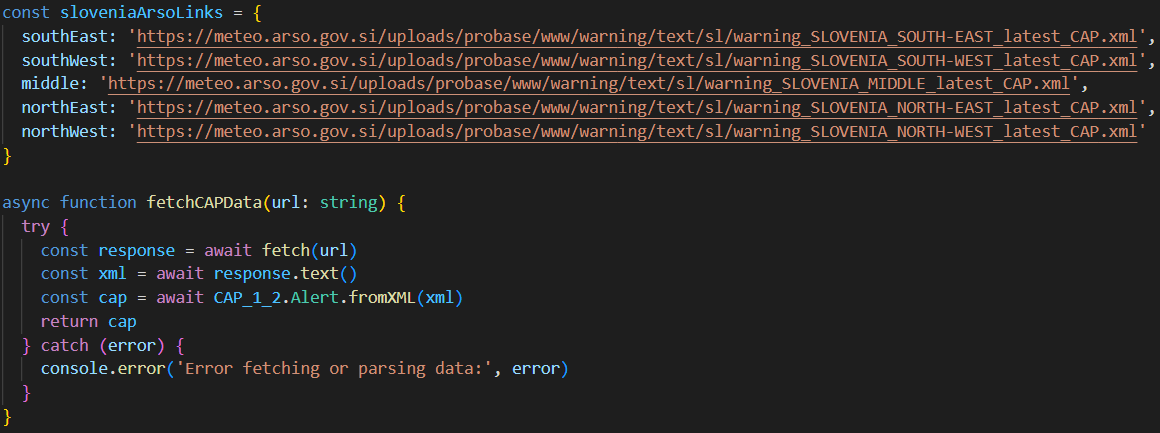
\includegraphics[width=0.7\textwidth]{images/arsoapi.png}
	      	\caption{Zunanji API}
	      	\label{fig:api}
	      \end{figure}
	      
	\item \textbf{Preverjanje zdravja}
	      \begin{itemize}
	      	\item Vsaki storitvi je dodana končna točka `/healthz`, ki preverja zdravje aplikacije.
	      	\item Kubernetes manifest je konfiguriran tako, da preverja zdravje storitev.
	      \end{itemize}
	\item \textbf{GraphQL}
	      \begin{itemize}
	      	\item Dodana je GraphQL podpora v Web mikrostoritvi.
	      	\item Dodana je GraphQL podpora v Notification mikrostoritvi.
	      \end{itemize}
	      
	      \begin{figure}[h!]
	      	\centering
	      	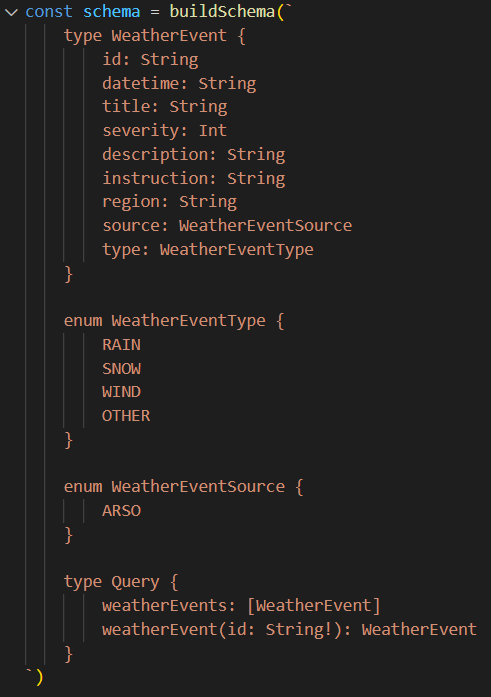
\includegraphics[width=0.4\textwidth]{images/graphql.png}
	      	\caption{GraphQL Shema}
	      	\label{fig:graphql}
	      \end{figure}
	      
	      \newpage
	      
	\item \textbf{Sporočilni sistem}
	      \begin{itemize}
	      	\item Dodan je RabbitMQ sporočilni sistem.
	      	\item Mikrostoritve Notification, Scraper in Storage komunicirajo preko RabbitMQ.
	      \end{itemize}
	      
	      \begin{figure}[h!]
	      	\centering
	      	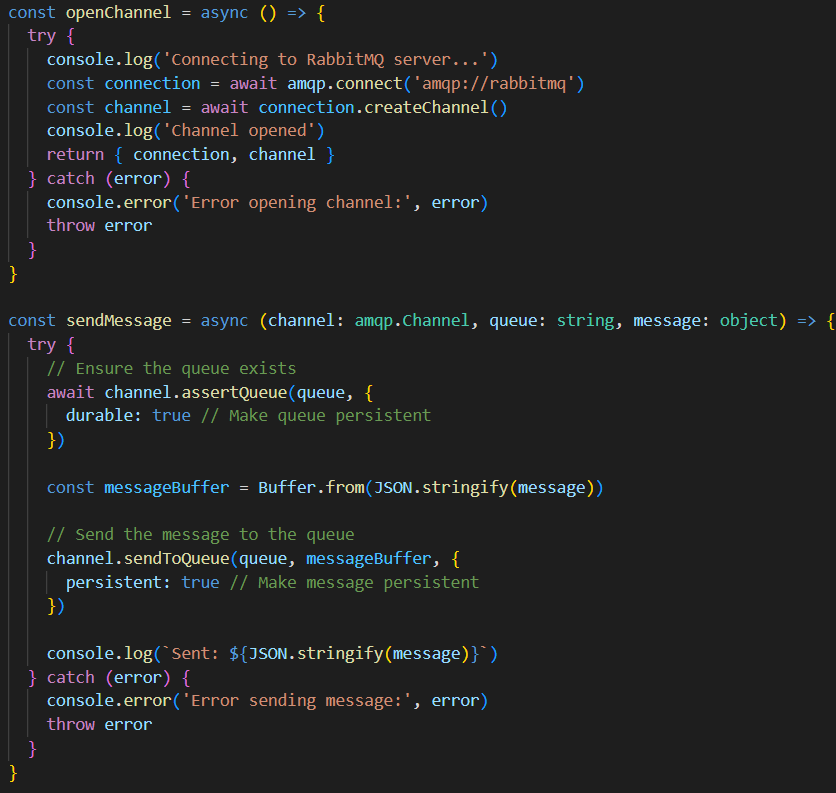
\includegraphics[width=0.5\textwidth]{images/rabbitmq.png}
	      	\caption{RabbitMQ koda}
	      	\label{fig:rabbitmq}
	      \end{figure}
	              
	\item \textbf{Grafični vmesnik}
	      \begin{itemize}
	      	\item Dodan je grafični vmesnik v Web mikrostoritvi.
	      	\item Vsebuje več podstrani.
	      	\item Za dostop do podatkov uporablja REST API.
	      \end{itemize}
	      
	      
	      \begin{figure}[h!]
	      	\centering
	      	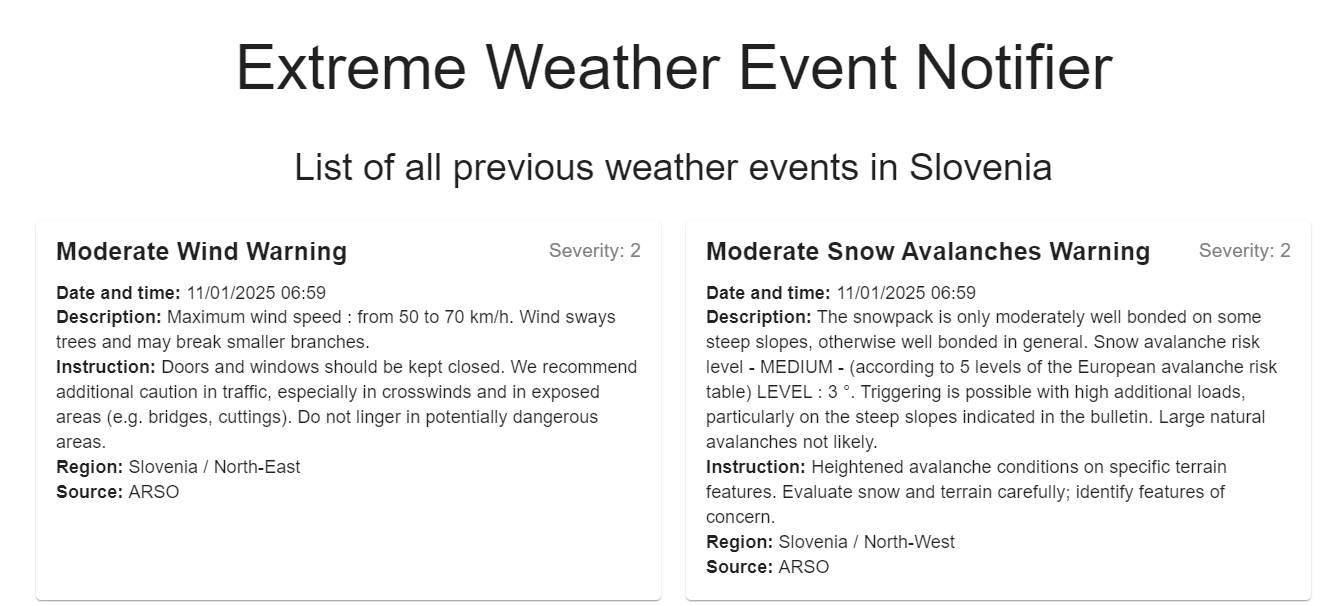
\includegraphics[width=0.7\textwidth]{images/web.png}
	      	\caption{Grafični vmesnik}
	      	\label{fig:web}
	      \end{figure}
	              
	\item \textbf{Ingress Controller}
	      \begin{itemize}
	      	\item Dodan je Ingress Controller, ki omogoča javni dostop do aplikacije.
	      	\item Implementiran je TLS/SSL samopodpisani certifikat.
	      \end{itemize}
	      
	      \begin{figure}[h!]
	      	\centering
	      	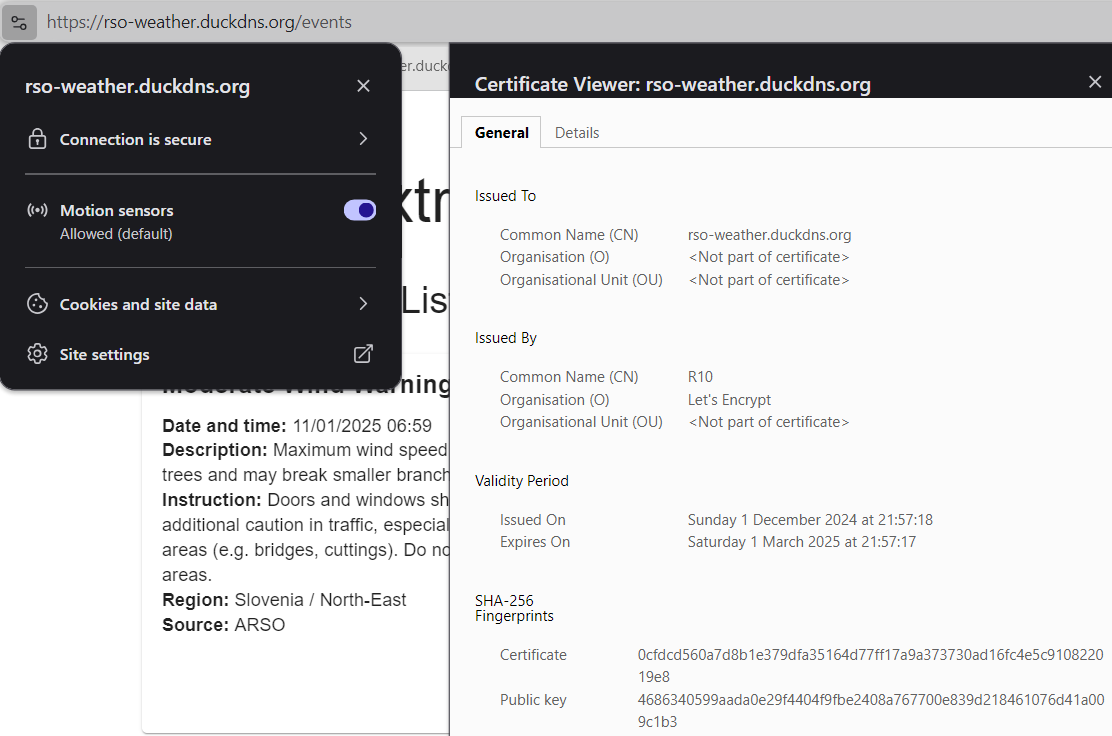
\includegraphics[width=0.7\textwidth]{images/ssl.png}
	      	\caption{SSL certifikat}
	      	\label{fig:ssl}
	      \end{figure}
\end{itemize}

\end{document}